\chapter{El software IRAF}
En esta clase revisaremos algunos de los comandos básicos de IRAF para la reducción de datos CCD. Esta será una guía bastante simple para comprender cómo se eliminan los ruidos debido a la instrumentación. Primero lo instalaremos en cualquier distribución de GNU/Linux y luego revisaremos algunos comandos básicos. 

\section{IRAF en GNU/Linux}
IRAF está disponible para sistemas Unix y por fortuna, existe una forma muy fácil de instalarlo en GNU/Linux. Acá se presentarán dos formas de instalarlo. Solo debes intentarlo de una de las dos formas disponibles, preferiblemente usando la primera. La segunda opción es únicamente si la primera falla.

Para instalar cualquier programa en las distribuciones de GNU/Linux basadas en Debian, se utiliza la herramienta \emph{Advanced Package Tool}, abreviada como \mintbold{shell}{apt}. Es posible instalar IRAF usando esta herramienta. Primero debemos actualizar nuestro sistema. Para eso necesitamos permisos de administrador.

Los permisos de administrador se obtienen con el comando \mintbold{shell}{sudo} (que proviene del inglés \textbf{s}witch \textbf{u}ser and \textbf{do}). Cada vez que usemos este comando nos pedirá ingresar nuestra contraseña. 

Abre una nueva terminal y actualiza tu sistema con el siguiente comando:

\begin{bash}
astronomer@PC:~ $ sudo apt update  
\end{bash}

El comando anterior pedirá que ingreses tu contraseña. Ahora puedes aplicar el siguiente comando:

\begin{bash}
astronomer@PC:~ $ sudo apt upgrade
\end{bash}

El comando anterior te pedirá que confirmes la acción escribiendo la letra <<\texttt{y}>> o <<\texttt{Y}>> y presionando la tecla Enter. Posteriormente instalará las actualizaciones a tu sistema. Esto puede tomar un poco de tiempo. 

\subsection{Instalación usando IRAF-Community}
Cuando tu sistema esté actualizado, debes instalar algunas dependencias para asegurar que la instalación de IRAF sea exitosa:

\begin{bash}
astronomer@PC:~ $ sudo apt install gcc make bison flex zlib1g-dev libreadline-dev
\end{bash}

Cuando la instalación termine, se debe instalar el programa \mintinline{shell}{git}:

\begin{bash}
astronomer@PC:~ $ sudo apt install git
\end{bash}
Ahora debes <<clonar>> el repositorio de IRAF-Community usando \texttt{git}:

\begin{bash}
astronomer@PC:~ $ git clone https://github.com/iraf-community/iraf.git
\end{bash}

Cuando el proceso termine, debes acceder al directorio que acabas de clonar:
\begin{bash}
astronomer@PC:~ $ cd iraf/
astronomer@PC:~/iraf $
\end{bash}

Ahora puedes compilar IRAF en tu sistema, para eso utiliza el siguiente comando:

\begin{bash}
astronomer@PC:~/iraf $ make 2>&1 | tee build.log
\end{bash}

Este proceso tomará varios minutos. Cuando termine, ejecuta el siguiente comando para hacer algunas pruebas sobre la instalación:

\begin{bash}
astronomer@PC:~/iraf $ make test
\end{bash}

El resultado debería verse similar a este:
\begin{bash}
ecl.e: README.md
ecl.e: files.md ......
ecl.e: images.imcoords.md ...........
ecl.e: images.imfilter.md .x............
ecl.e: images.imfit.md ...
ecl.e: images.imgeom.md ........
ecl.e: images.immatch.md ..
ecl.e: lists.md .......
ecl.e: noao.astutil.md ........
ecl.e: noao.digiphot.photcal.md .
ecl.e: numerical-recipes.md ..........
ecl.e: os.md ..
ecl.e: programming.md ............
ecl.e: sys.vops.md .
ecl.e: test-syntax.md ...xs.
ecl.e: testproc.md ..........................
ecl.e: utilities.nttools.md ..............
Test summary:  128 passed
   1 skipped
   2 xfailed
\end{bash}

Finalmente, para terminar la instalación, ejecuta el siguiente comando:

\begin{bash}
astronomer@PC:~/iraf $ sudo make install
\end{bash}

Con eso, el sistema tendrá la configuración necesaria para usar IRAF. Una vez que el proceso termine, puedes cerrar la terminal y abrir una nueva. 

En una nueva terminal debes ejecutar el siguiente comando:
\begin{bash}
astronomer@PC:~ $ mkiraf
\end{bash}

Esto creará una carpeta llamada <<\texttt{uparm}>> en tu directorio actual. En este caso, se creó dicha carpeta en el directorio personal. El siguiente comando debe ejecutarse en el mismo directorio donde se encuentra la carpeta \texttt{uparm} para que IRAF funcione correctamente:

\begin{bash}
astronomer@PC:~ $ ecl
\end{bash}

El comando abrirá la interfaz de IRAF en la terminal. Esta interfaz puede no ser muy amigable, así que adicionalmente se instalará otra interfaz, llamada <<\mintinline{shell}{pyraf}>>. Esto puedes hacerlo con el siguiente comando:

\begin{bash}
astronomer@PC:~ $ pip install pyraf
\end{bash}

Cuando la instalación termine, debes ejecutar el comando \mintinline{shell}{pyraf} para comenzar a usar IRAF en la interfaz de pyraf. Los detalles se verán más adelante.

\subsection{Instalación usando astroconda}
De manera alternativa, puedes instalar IRAF y \texttt{pyraf} usando \texttt{anaconda}/\texttt{miniconda}. Primero debes activar tu ambiente de conda. Una vez que lo hayas hecho, agrega el canal de AstroConda:

\begin{bash}
(base) astronomer@PC:~ $ conda config --add channels http://ssb.stsci.edu/astroconda
\end{bash}

Posteriormente, crea un nuevo entorno virtual con el cual usarás IRAF/Pyraf:

\begin{bash}
(base) astronomer@PC:~ $ conda create -n iraf27 python=2.7 iraf-all pyraf-all stsci
\end{bash}

Ahora activa tu entorno de IRAF:
\begin{bash}
(base) astronomer@PC:~ $ conda activate iraf27
(iraf27) astronomer@PC:~ $ 
\end{bash}
Desplázate a tu carpeta de trabajo y ejecuta el comando 
\begin{bash}
(iraf27) astronomer@PC:~ $ mkiraf
\end{bash}
Esto creará una carpeta llamada <<\texttt{uparm}>>. Ahora puedes ejecutar el comando \texttt{pyraf} para comenzar a usar IRAF con la interfaz de Pyraf:

\begin{bash}
(iraf27) astronomer@PC:~ $ pyraf
\end{bash}

Ten en cuenta que para que las cosas funcionen correctamente, el comando \texttt{pyraf} debe ejecutarse en el directorio donde se encuentre ubicada la carpeta \texttt{uparm}. 

\subsection{Lanzando la interfaz}
Vale la pena aclarar un punto antes de continuar: IRAF es el software que contiene las herramientas necesarias para realizar las tareas de calibración de imágenes CCD. IRAF tiene su propia interfaz para que sea utilizada desde la terminal, pero podría resultar poco amigable a los usuarios nuevos. En cambio, Pyraf es una interfaz gráfica para usar dichas herramientas, debido a eso, utilizaremos Pyraf. Pero ten en cuenta que la única diferencia entre IRAF y Pyraf es la interfaz gráfica, ambos utilizan las mismas herramientas de IRAF. 

A pesar que utilizaremos Pyraf, vale la pena mostrar cómo se lanza la interfaz por defecto de IRAF, por si en algún momento quieres aprender a utilizarla. Anteriormente cuando instalamos IRAF, ejecutamos el comando \norbash{mkiraf}. Dicho comando generó una carpeta llamada \norbash{uparm}. Para que IRAF fucnione correctamente, sin importar si usamos Pyraf o IRAF, debemos lanzar el software desde el directorio donde está ubicado \norbash{uparm}. 

Por defecto, realizamos la instalación en la carpeta personal. Por lo tanto, la carpeta \norbash{uparm} debería estar en dicho directorio. Para usar IRAF entonces, es suficiente lanzar una nueva terminal y escribir el comando <<\norbash{ecl}>>. En la Figura \ref{fig:ecl-output} se muestra el resultado de ejecutar el comando.

\begin{figure}[htb]
  \centering
	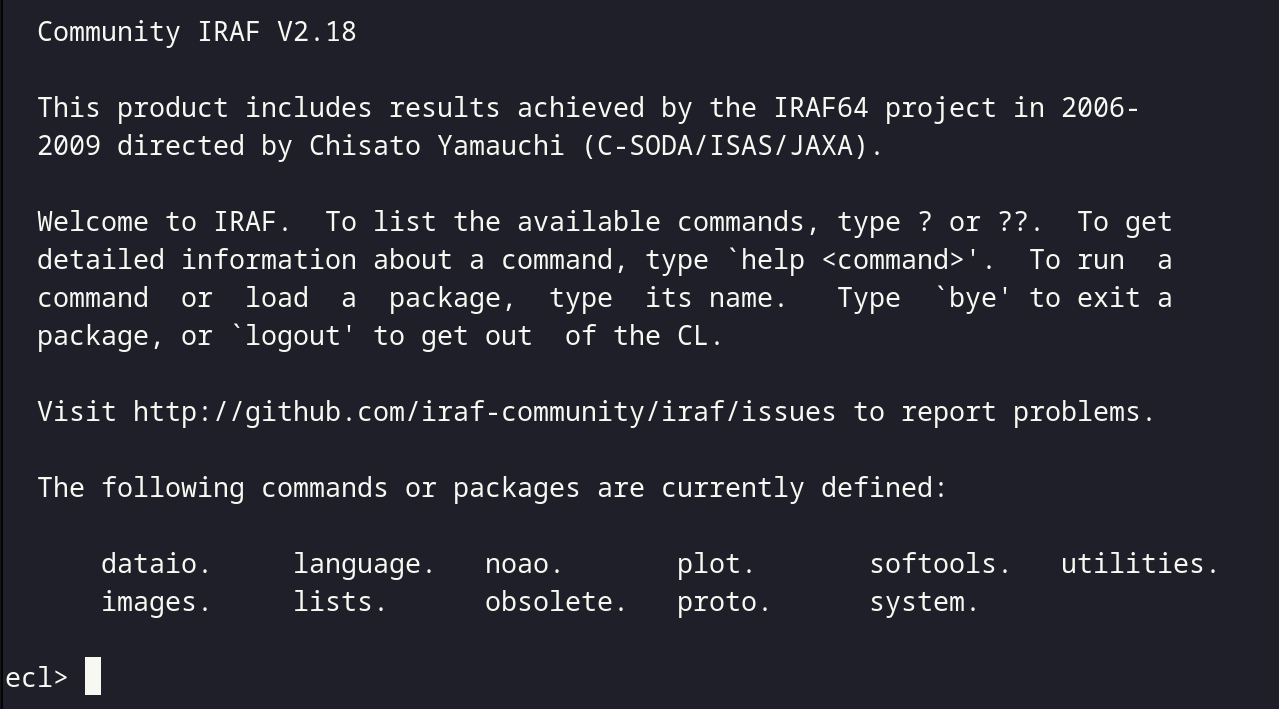
\includegraphics[width=\textwidth]{figures/ecl-output.png}
	\caption{Mensaje que se muestra al ejecutar el comando \norbash{ecl}.}
	\label{fig:ecl-output} 
\end{figure}

En este ambiente, los caracteres <<\norbash{ecl>}>> nos indican que IRAF está listo para recibir comandos e instrucciones. Para accedder a las herramientas de reducción de datos, debemos escribir y ejecutar el comando <<\norbash{imred}>> (que proviene de \emph{image reduction}):

\begin{bash}
ecl> imred
      argus.       dtoi.        irred.       specred.
      bias.        echelle.     irs.         vtel.
      ccdred.      generic.     kpnocoude.   
      crutil.      hydra.       kpnoslit.    
      ctioslit.    iids.        quadred.     

imred> 
\end{bash}

El comando \norbash{imred} desplegó una lista de las herramientas disponibles para la reducción de imágenes. Las que utilizaremos se encuentran dentro de la opción llamada <<\norbash{ccdred}>>. Por lo tanto, debemos ejecutarlo:

\begin{bash}
imred> ccdred
      badpiximage       ccdproc           mkillumcor
      ccdgroups         ccdtest.          mkillumflat
      ccdhedit          combine           mkskycor
      ccdinstrument     darkcombine       mkskyflat
      ccdlist           flatcombine       setinstrument
      ccdmask           mkfringecor       zerocombine

ccdred>
\end{bash}

Nota cómo el prompt cambia cada vez que ejecutamos un comando. Las herramientas que nos interesan dentro de \norbash{ccdred} son: \norbash{zerocombine}, \norbash{darkcombine}, \norbash{flatcombine} y \norbash{combine}. La tarea \norbash{zerocombine} se utiliza para combinar las imágenes de bias, recuerda que a este proceso se le suele llamar corrección de nivel cero. Lo recomendable para usar cualquiera de esas tareas es primero revisar sus parámetros. Esto se logra con el comando <<\norbash{lpar}>> (que proviene de las palabras \emph{list parameters} en inglés) seguido del nombre de la tarea. Por ejemplo, revisemos los parámetros de \norbash{zerocombine}:

\begin{bash}
ccdred> lpar zerocombine
        input =                 List of zero level images to combine
      (output = "Zero")         Output zero level name
     (combine = "average")      Type of combine operation
      (reject = "minmax")       Type of rejection
     (ccdtype = "zero")         CCD image type to combine
     (process = no)             Process images before combining?
      (delete = no)             Delete input images after combining?
     (clobber = no)             Clobber existing output image?
       (scale = "none")         Image scaling
     (statsec = "")             Image section for computing statistics
        (nlow = 0)              minmax: Number of low pixels to reject
       (nhigh = 1)              minmax: Number of high pixels to reject
       (nkeep = 1)              Minimum to keep (pos) or maximum to reject (neg)
       (mclip = yes)            Use median in sigma clipping algorithms?
      (lsigma = 3.)             Lower sigma clipping factor
      (hsigma = 3.)             Upper sigma clipping factor
     (rdnoise = "0.")           ccdclip: CCD readout noise (electrons)
        (gain = "1.")           ccdclip: CCD gain (electrons/DN)
      (snoise = "0.")           ccdclip: Sensitivity noise (fraction)
       (pclip = -0.5)           pclip: Percentile clipping parameter
       (blank = 0.)             Value if there are no pixels
        (mode = "ql")           
ccdred> 
\end{bash}

El comando \norbash{lpar} únicamente nos muestra una lista de los parámetros disponibles para las tareas. Para editarlos, debemos utilzar el comando <<\norbash{epar}>> (que proviene de las palabras \emph{edit parameters} en inglés) seguido del nombre de la tarea. La salida de dicho parámetro es muy similar a la de \norbash{lpar}, con la diferencia que permite editar cada campo. Para guardar los cambios y salir, se deben ejecutar el comando <<\norbash{:q}>>.

Lo importante de la lista de parámetros mostrados anteriormente, es la entrada (o input), la cual puede ser una sola imagen con extensión \norbash{.fits} o toda una lista de imágenes. Para mostrar las ventajas de la interfaz de Pyraf, repitamos los pasos anteriores pero ahora usando Pyraf. 

Cierra la terminal que estás usando y abre una nueva. Ya que la carpeta \norbash{uparm} está en tu directorio personal, puedes ejecutar directamente el comando \norbash{pyraf} al momento de abrir la nueva terminal. Notarás que la interfaz se ve muy parecida a la anterior, con la única diferencia que en lugar de los caracteres \norbash{ecl>}, ahora se muestra una flecha: \norbash{-->} en el prompt. 

Ahora escribre uno tras otro los comandos \norbash{imred}, \norbash{ccdred}, \norbash{epar zerocombine}:

\begin{bash}
imred/:
 argus/         ctioslit/       hydra/          kpnocoude/      vtel/
 bias/          dtoi/           iids/           kpnoslit/
 ccdred/        echelle/        irred/          quadred/
 crutil/        generic/        irs/            specred/
--> ccdred
ccdred/:
 badpiximage    ccdlist         combine         mkillumcor      setinstrument
 ccdgroups      ccdmask         darkcombine     mkillumflat     zerocombine
 ccdhedit       ccdproc         flatcombine     mkskycor
 ccdinstrument  ccdtest         mkfringecor     mkskyflat
--> epar zerocombine
\end{bash}

La gra diferencia es que al editar parámetros, se muestra una interfaz gráfica mucho más fácil de usar comparada con la terminal. Esto se muestra en la Figura \ref{fig:pyraf-epar-example}.

\begin{figure}[htb]
  \centering
	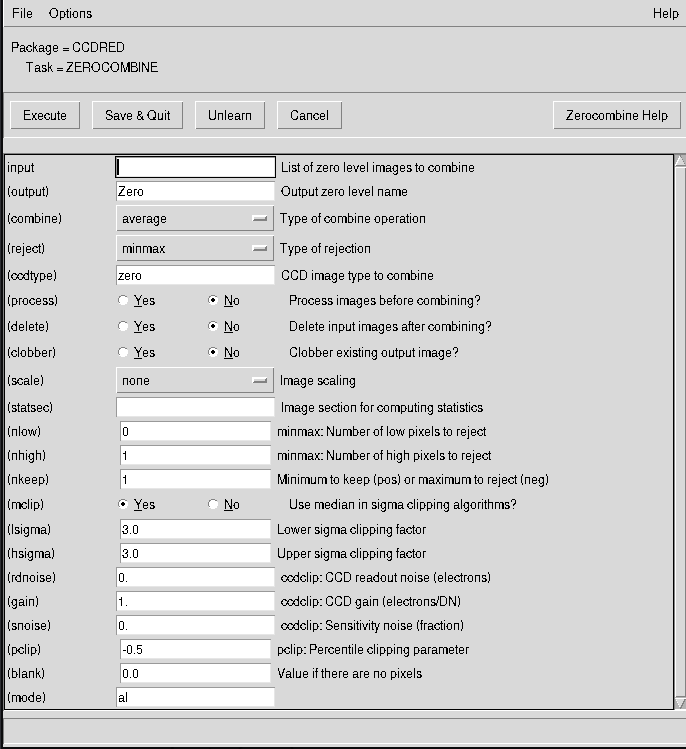
\includegraphics[width=0.7\textwidth]{figures/pyraf-epar-example.png}
	\caption{Interfaz gráfica para editar parámetros en Pyraf}
	\label{fig:pyraf-epar-example} 
\end{figure}


La lista de parámetros en las otras tareas mencionadas: \norbash{darkcombine}, \norbash{flatcombine} y \norbash{combine} son muy similares y las revisaremos con detalle en la siguiente clase. 
